\documentclass[12pt]{article}
\usepackage{graphicx}
\usepackage{caption}
\usepackage{geometry}
\usepackage{listings}
\usepackage{amsthm}
\geometry{margin=1in}
\RequirePackage{amsmath}
\usepackage{cite}
\usepackage{amsmath,amssymb,amsfonts,amsthm}
\usepackage{algorithmic}
\usepackage{textcomp}
\usepackage{xcolor}
\usepackage{txfonts}
\usepackage{enumitem}
\usepackage{mathtools}
\usepackage{gensymb}
\usepackage{comment}
\usepackage[breaklinks=true]{hyperref}
\usepackage{tkz-euclide} 
\usepackage{listings}                                                            \usepackage[utf8]{inputenc}     
\usepackage{xparse}
\usepackage{color}                                            
\usepackage{array}                                            
\usepackage{longtable}                                       
\usepackage{calc}                                             
\usepackage{multirow}
\usepackage{multicol}
\usepackage[version=4]{mhchem} 
\usepackage{hhline}                                           
\usepackage{ifthen}                                           
\usepackage{lscape}
\usepackage{tabularx}
\usepackage{array}
\usepackage{float}
\usepackage{gvv}
\usepackage{gvv-book}

\author{EE25BTECH11010-ARSH DHOKE}
\title{GATE 2012 Questions}
\date{}

\begin{document}
\maketitle

\textbf{Q.1- Q.25 carry one mark each}
\begin{enumerate}

\item In the proton decoupled $^{13}$C NMR spectrum of 7-norbornanone, the number of signals obtained is  
\begin{enumerate}
\begin{multicols}{2}
    \item 7 
    \item 3 
    \item 4 
    \item 5
\end{multicols}  
\end{enumerate}
\hfill (GATE CY 2012)

\item Identify the most probable product in the given reaction  
\begin{figure}[H]
    \centering
    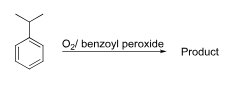
\includegraphics[width=0.4\columnwidth]{figs/q2.png}
    \caption{Figure for Q.2}
    \label{fig:q2}
\end{figure}
\begin{enumerate}
\begin{figure}[H]
    \item 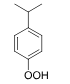
\includegraphics[width=0.12\columnwidth]{figs/q2a.png}
    \caption{Option A}
    \label{fig:q2a}
    \item 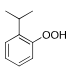
\includegraphics[width=0.12\columnwidth]{figs/q2b.png}
    \caption{Option B}
    \label{fig:q2b}
    \item 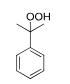
\includegraphics[width=0.12\columnwidth]{figs/q2c.png}
    \caption{Option C}
    \label{fig:q2c}
    \item 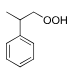
\includegraphics[width=0.12\columnwidth]{figs/q2d.png}
    \caption{Option D}
    \label{fig:q2d}
\end{figure}
\end{enumerate}
\hfill (GATE CY 2012)


\item In the cyclization reaction given below, the most probable product formed is  
\begin{figure}[H]
    \centering
    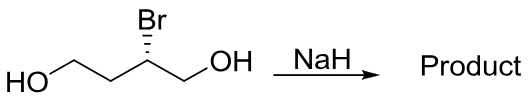
\includegraphics[width=0.4\columnwidth]{figs/q3.png}
\end{figure}
\begin{enumerate}
\begin{figure}[H]
    \item 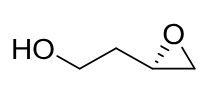
\includegraphics[width=0.12\columnwidth]{figs/q3a.png}
    \caption{Option A}
    \label{fig:q3a}
    \item 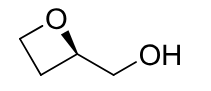
\includegraphics[width=0.12\columnwidth]{figs/q3b.png}
    \caption{Option B}
    \label{fig:q3b}
    \item 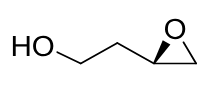
\includegraphics[width=0.12\columnwidth]{figs/q3c.png}
    \caption{Option C}
    \label{fig:q3c}
    \item 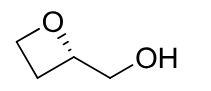
\includegraphics[width=0.12\columnwidth]{figs/q3d.png}
    \caption{Option D}
    \label{fig:q3d}
\end{figure}
\end{enumerate}
\hfill (GATE CY 2012)

\item If $\Delta y$ and $\Delta p_y$ are the uncertainties in the y-coordinate and the y component of the momentum of a particle respectively, then, according to uncertainty principle  
\[
\Delta y \Delta p_y \geq \frac{h}{2\pi}
\]  
where $h$ is Planck’s constant.  
\begin{multicols}{2}
\begin{enumerate}
    \item $\geq h$ 
    \item $> h/2$ 
    \item $> h$ 
    \item $\geq h/2$
\end{enumerate}
\end{multicols}
\hfill (GATE CY 2012)

\item The average length of a typical $\alpha$-helix comprised of 10 amino acids is  
\begin{enumerate}
\begin{multicols}{2}
    \item 10 \AA 
    \item 15 \AA 
    \item 36 \AA 
    \item 54 \AA
\end{multicols}
\end{enumerate}
\hfill (GATE CY 2012)

\item Number of thymine residues in a 5000 kb DNA containing 23\% guanine residues is  
\begin{enumerate}
\begin{multicols}{2}
    \item $2.70 \times 10^8$ 
    \item $2.70 \times 10^7$ 
    \item $1.35 \times 10^6$ 
    \item $1.35 \times 10^7$
\end{multicols}
\end{enumerate}
\hfill (GATE CY 2012)

\item Shown below is a Hammett plot obtained for the reaction

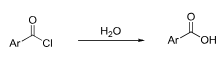
\includegraphics[width=0.45\columnwidth]{figs/q7a.png} 

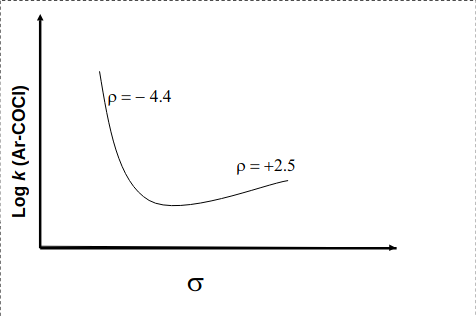
\includegraphics[width=0.45\columnwidth]{figs/q7.png}  

The change in slope of the plot indicates that  
\begin{enumerate}
    \item the reaction does not follow linear free energy relationship
    \item electrons are being withdrawn from the transition state in the mechanism
    \item electrons are being donated to the transition state in the mechanism
    \item the mechanism of the reaction is changing
\end{enumerate}
\hfill (GATE CY 2012)

\item The ratio of relative intensities of the two molecular ion peaks of methyl bromide (CH$_3$Br) in the mass spectrum is  

\begin{enumerate}
\begin{multicols}{2}
    \item M$^+$ : (M+2)$^+$ = 1:3
    \item M$^+$ : (M+2)$^+$ = 3:1
    \item M$^+$ : (M+2)$^+$ = 1:1
    \item M$^+$ : (M+2)$^+$ = 1:2
\end{multicols}
\end{enumerate}
\hfill (GATE CY 2012)

\item A disaccharide that will not give Benedict’s test and will not form osazone is  
\begin{multicols}{2}
\begin{enumerate}
    \item maltose
    \item lactose
    \item cellobiose
    \item sucrose
\end{enumerate}
\end{multicols}
\hfill (GATE CY 2012)

\item Choose the allowed transition  
\begin{multicols}{2}
\begin{enumerate}
    \item $^{1}\Sigma_{u}^{+} \rightarrow ^{3}\Sigma_{g}^{+}$
    \item $^{1}\Sigma_{u}^{+} \rightarrow ^{1}\Sigma_{u}^{+}$
    \item $^{1}\Sigma_{u}^{+} \rightarrow ^{1}\Sigma_{g}^{+}$
    \item $^{1}\Sigma_{u}^{+} \rightarrow ^{3}\Sigma_{u}^{+}$
\end{enumerate}
\end{multicols}
\hfill (GATE CY 2012)

\item The angular part of the wavefunction for the electron in a hydrogen atom is proportional to  
\[
\sin^2 \theta \cos \theta \, e^{2i\phi}
\]  
The values of the azimuthal quantum number ($l$) and the magnetic quantum number ($m$) are, respectively  
\begin{multicols}{2}
\begin{enumerate}
    \item 2 and 2
    \item 2 and $-2$
    \item 3 and 2
    \item 3 and $-2$
\end{enumerate}
\end{multicols}
\hfill (GATE CY 2012)

\item Let $\phi_{2p_z}^C$ and $\phi_{2p_x}^C$ denote the wavefunctions of the 2p$_z$ and 2p$_x$ orbitals of carbon, respectively, and $\phi_{2p_z}^O$ and $\phi_{2p_x}^O$ represent the wavefunctions of the 2p$_z$ and 2p$_x$ orbitals of oxygen, respectively. If $c_1$ and $c_2$ are constants used in linear combinations and the CO molecule is oriented along the z-axis, then, according to molecular orbital theory, the $\pi$-bonding molecular orbital has a wavefunction given by  
\begin{multicols}{2}
\begin{enumerate}
    \item $c_1 \phi_{2p_x}^C + c_2 \phi_{2p_x}^O$
    \item $c_1 \phi_{2p_z}^C + c_2 \phi_{2p_z}^O$
    \item $c_1 \phi_{2p_x}^C + c_2 \phi_{2p_z}^O$
    \item $c_1 \phi_{2p_z}^C + c_2 \phi_{2p_x}^O$
\end{enumerate}
\end{multicols}
\hfill (GATE CY 2012)

\item The bond that gives the most intense band in the infrared spectrum for its stretching vibration is  
\begin{multicols}{2}
\begin{enumerate}
    \item C–H
    \item N–H
    \item O–H
    \item S–H
\end{enumerate}
\end{multicols}
\hfill (GATE CY 2012)

\item If $x_A$ and $x_B$ are the respective mole fractions of A and B in an ideal solution of the two and $T_A, T_B, T$ are the fusion temperatures of pure A, pure B and the ideal solution respectively, then  

\begin{multicols}{2}
\begin{enumerate}
    \item $1 - x_B = \exp \brak{ \dfrac{-\Delta H^{\text{fus}}(B)}{R} \brak{ \dfrac{1}{T} - \dfrac{1}{T_B} } }$
    \item $1 - x_B = \exp \brak{ \dfrac{\Delta H^{\text{fus}}(A)}{R} \brak{ \dfrac{1}{T} - \dfrac{1}{T_A} } }$
    \item $1 - x_B = \exp \brak{ \dfrac{\Delta H^{\text{fus}}(B)}{R} \brak{ \dfrac{1}{T} - \dfrac{1}{T_B} } }$
    \item $1 - x_B = \exp \brak{ \dfrac{-\Delta H^{\text{fus}}(A)}{R} \brak{ \dfrac{1}{T} - \dfrac{1}{T_A} } }$
\end{enumerate}
\end{multicols}
\hfill (GATE CY 2012)

\item For a reaction involving two steps given below

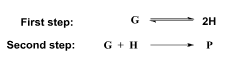
\includegraphics[width=0.4\columnwidth]{figs/q15.png}

Assume that the first step attains equilibrium rapidly. The rate of formation of P is proportional to
\begin{multicols}{2}
\begin{enumerate}
    \item $\brak{G}^{1/2}$
    \item $\brak{G}$
    \item $\brak{G}^{2}$
    \item $\brak{G}^{3/2}$
\end{enumerate}
\end{multicols}
\hfill (GATE CY 2012)

\item A metal chelate that can be used for separation and quantitative analysis of aluminium ions by gas chromatography is
\begin{multicols}{2}
\begin{enumerate}
    \item EDTA
    \item ethylene glycol
    \item dinonyl phthalate
    \item trifluoroacetylacetone
\end{enumerate}
\end{multicols}
\hfill (GATE CY 2012)

\item The enthalpies of hydration of $\mathrm{Ca^{2+}}$, $\mathrm{Mn^{4+}}$ and $\mathrm{Zn^{2+}}$ follow the order
\begin{multicols}{2}
\begin{enumerate}
    \item $\mathrm{Mn^{4+} > Ca^{2+} > Zn^{2+}}$
    \item $\mathrm{Zn^{2+} > Ca^{2+} > Mn^{4+}}$
    \item $\mathrm{Mn^{4+} > Zn^{2+} > Ca^{2+}}$
    \item $\mathrm{Zn^{2+} > Mn^{4+} > Ca^{2+}}$
\end{enumerate}
\end{multicols}
\hfill (GATE CY 2012)


\item The number of terminal carbonyl groups present in Fe$_2$(CO)$_9$ is
\begin{multicols}{2}
\begin{enumerate}
    \item 2
    \item 5
    \item 6
    \item 3
\end{enumerate}
\end{multicols}
\hfill (GATE CY 2012)

\item Among the following substituted silanes, the one that gives cross-linked silicone polymer upon hydrolysis is
\begin{multicols}{2}
\begin{enumerate}
    \item (CH$_3$)$_4$Si
    \item CH$_3$SiCl$_3$
    \item (CH$_3$)$_2$SiCl$_2$
    \item (CH$_3$)$_3$SiCl
\end{enumerate}
\end{multicols}
\hfill (GATE CY 2012)

\item The plot of $\chi T$ versus $T$ (where $\chi$ is molar magnetic susceptibility and $T$ is the temperature) for a paramagnetic complex which strictly follows Curie equation is
\begin{figure}[H]
\begin{enumerate}
    \item 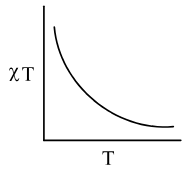
\includegraphics[width=0.2\columnwidth]{figs/q20a.png}
    \caption{Option A}
    \label{fig:q20a}
    \item 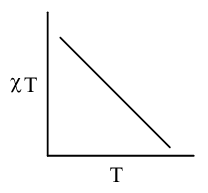
\includegraphics[width=0.2\columnwidth]{figs/q20b.png}
    \caption{Option B}
    \label{fig:q20b}
    \item 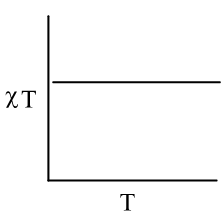
\includegraphics[width=0.2\columnwidth]{figs/q20c.png}
    \caption{Option C}
    \label{fig:q20c}
    \item 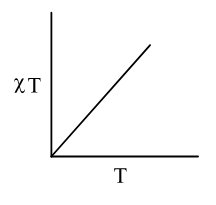
\includegraphics[width=0.2\columnwidth]{figs/q20d.png}
    \caption{Option D}
    \label{fig:q20d}
\end{enumerate}
\end{figure}
\hfill (GATE CY 2012)

\item Among the following donors, the one that forms most stable adduct with the Lewis acid B(CH$_3$)$_3$ is
\begin{multicols}{2}
\begin{enumerate}
    \item 4-methylpyridine
    \item 2,6-dimethylpyridine
    \item 4-nitropyridine
    \item 2,6-di-tert-butylpyridine
\end{enumerate}
\end{multicols}
\hfill (GATE CY 2012)

\item The complex with \textit{inverse}-spinel structure is
\begin{multicols}{2}
\begin{enumerate}
    \item Co$_3$O$_4$
    \item Fe$_3$O$_4$
    \item MgAl$_2$O$_4$
    \item Mn$_3$O$_4$
\end{enumerate}
\end{multicols}
\hfill (GATE CY 2012)

\item The IUPAC nomenclature of Na[PtCl$_6$] is
\begin{multicols}{2}
\begin{enumerate}
    \item sodium hexachlorophosphine(V)
    \item sodium hexachlorophosphate(V)
    \item sodium hexachlorophosphine
    \item sodium hexachlorophosphite(V)
\end{enumerate}
\end{multicols}
\hfill (GATE CY 2012)

\item An intermediate formed during the hydroformylation of olefins using Co$_2$(CO)$_8$ as catalyst is
\begin{multicols}{2}
\begin{enumerate}
    \item HCo(CO)$_6$
    \item H$_4$Co(CO)$_3$
    \item H$_2$Co(CO)$_4$
    \item HCo(CO)$_4$
\end{enumerate}
\end{multicols}
\hfill (GATE CY 2012)

\item The order of polarity of NH$_3$, NF$_3$ and BF$_3$ is
\begin{multicols}{2}
\begin{enumerate}
    \item NH$_3 <$ NF$_3 <$ BF$_3$
    \item BF$_3 <$ NF$_3 <$ NH$_3$
    \item BF$_3 <$ NH$_3 <$ NF$_3$
    \item NF$_3 <$ BF$_3 <$ NH$_3$
\end{enumerate}
\end{multicols}
\hfill (GATE CY 2012)

\textbf{Q.26 to Q.55 carry two marks each.}

\item From a carboxymethyl-cellulose column at pH 6.0, arginine, valine and glutamic acid will elute in the order
\begin{multicols}{2}
\begin{enumerate}
    \item arginine, valine, glutamic acid
    \item arginine, glutamic acid, valine
    \item glutamic acid, arginine, valine
    \item glutamic acid, valine, arginine
\end{enumerate}
\end{multicols}
\hfill (GATE CY 2012)

\item Symmetry operations of the four C$_2$ axes perpendicular to the principal axis belong to the same class in the point group(s)
\begin{multicols}{2}
\begin{enumerate}
    \item D$_4$
    \item D$_{4d}$
    \item D$_{4h}$
    \item D$_{4h}$ and D$_{4d}$
\end{enumerate}
\end{multicols}
\hfill (GATE CY 2012)

\item At 298 K, the EMF of the cell
\[
\text{Pt} \;|\; \text{H}_2(1\;\text{bar}) \;|\; \text{H}^+(\text{solution}) \;||\; \text{Cl}^- \;|\; \text{Hg}_2\text{Cl}_2 \;|\; \text{Hg}
\]
is 0.7530 V. The standard potential of the calomel electrode is 0.2802 V. If the liquid junction potential is zero, the pH of the solution is
\begin{multicols}{2}
\begin{enumerate}
    \item 4.7
    \item 7.4
    \item 8.0
    \item 12.7
\end{enumerate}
\end{multicols}
\hfill (GATE CY 2012)

\item The wavefunction of a 1-D harmonic oscillator between $x = +\infty$ and $x = -\infty$ is given by 
\[
\psi(x) = N(2x^2 - 1)e^{-x^2/2}.
\] 
The value of $N$ that normalizes the function $\psi(x)$ is 

\[
\text{(Given: } \int_{-\infty}^{\infty} x^{2n} e^{-x^2} dx = \frac{1 \cdot 3 \cdot 5 \cdots (2n-1)}{2^n} \sqrt{\pi} \,)
\]

\begin{enumerate}
    \item $\brak{\dfrac{1}{8\sqrt{\pi}}}^{1/2}$
    \item $\brak{\dfrac{1}{3\sqrt{\pi}}}^{1/2}$
    \item $\brak{\dfrac{1}{2\sqrt{\pi}}}^{1/2}$
    \item $\brak{\dfrac{1}{4\sqrt{\pi}}}^{1/2}$
\end{enumerate}
\hfill (GATE CY 2012)


\item Consider the reaction 
\[
\text{H}_2 + \text{C}_2\text{H}_4 \to \text{C}_2\text{H}_6
\]

The molecular diameters of H$_2$ and C$_2$H$_4$ are 1.8 \AA{} and 3.6 \AA{} respectively.  
The pre-exponential factor in the rate constant calculated using collision theory in m$^3$(mole)$^{-1}$s$^{-1}$ is approximately

\[
\left( \text{For this reaction at 300 K, } \brak{\frac{8k_B T}{\pi \mu}}^{1/2}, \quad N_A = 1.11 \times 10^{27}\, m(\text{mole})^{-1} s^{-1} \text{, where the symbols have their usual meanings} \right)
\]

\begin{multicols}{2}
\begin{enumerate}
    \item $2.5 \times 10^8$
    \item $2.5 \times 10^{14}$
    \item $9.4 \times 10^{17}$
    \item $9.4 \times 10^{23}$
\end{enumerate}
\end{multicols}
\hfill (GATE CY 2012)


\item The molecular partition function of a system is given by
\[
q(T) = \brak{\frac{k_B T}{hc}}^{3/2} \brak{\frac{8 \pi^2 m k_B T}{h^2}}^{3/2},
\]
where the symbols have their usual meanings.  

The heat capacity at constant volume for this system is

\begin{multicols}{2}
\begin{enumerate}
    \item 3R
    \item 6R
    \item 9R/2
    \item 3R/2
\end{enumerate}
\end{multicols}
\hfill (GATE CY 2012)

\item Consider the phase diagram given below.  

\begin{figure}[H]
    \centering
    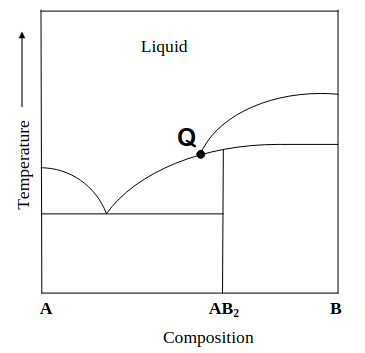
\includegraphics[width=0.45\columnwidth]{figs/q32.png}
    \caption{Figure for Q.32}
    \label{fig:q32}
\end{figure}

At the intersection point Q the phases that are in equilibrium are  

\begin{enumerate}
    \item solid A, solid B and solid AB$_2$
    \item solid A, solid AB$_2$ and liquid
    \item solid B, solid AB$_2$ and liquid
    \item solid A, solid B, solid AB$_2$ and liquid
\end{enumerate}
\hfill (GATE CY 2012)


\item Identify the product from the following reaction  

\begin{figure}[H]
    \centering
    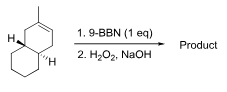
\includegraphics[width=0.4\columnwidth]{figs/q33.png}
    \caption{Figure for Q.33}
    \label{fig:q33}
\end{figure}

(9-BBN = 9-Borabicyclo[3.3.1]nonane)  

\begin{figure}[H]
\centering
\begin{enumerate}
    \item 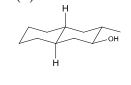
\includegraphics[width=0.18\columnwidth]{figs/q33a.png}
    \caption{Option A}
    \label{fig:q33a}
    \item 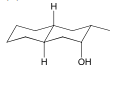
\includegraphics[width=0.18\columnwidth]{figs/q33b.png}
    \caption{Option B}
    \label{fig:q33b}
    \item 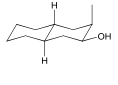
\includegraphics[width=0.18\columnwidth]{figs/q33c.png}
    \caption{Option C}
    \label{fig:q33c}
    \item 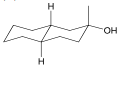
\includegraphics[width=0.18\columnwidth]{figs/q33d.png}
    \caption{Option D}
    \label{fig:q33d}
\end{enumerate}
\end{figure}
\hfill (GATE CY 2012)

\item The product from the following reaction is  

\begin{figure}[H]
    \centering
    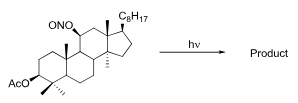
\includegraphics[width=0.45\columnwidth]{figs/q34.png}
    \caption{Figure for Q.34}
    \label{fig:q34}
\end{figure}

\begin{figure}[H]
\centering
\begin{enumerate}
    \item 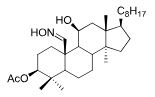
\includegraphics[width=0.25\columnwidth]{figs/q34a.png}
    \caption{Option A}
    \label{fig:q34a}
    \item 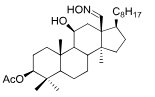
\includegraphics[width=0.25\columnwidth]{figs/q34b.png}
    \caption{Option B}
    \label{fig:q34b}
    \item 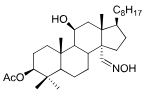
\includegraphics[width=0.25\columnwidth]{figs/q34c.png}
    \caption{Option C}
    \label{fig:q34c}
    \item 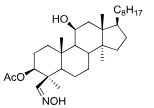
\includegraphics[width=0.25\columnwidth]{figs/q34d.png}
    \caption{Option D}
    \label{fig:q34d}
\end{enumerate}
\end{figure}
\hfill (GATE CY 2012)


\item The acid catalyzed cyclization of 5-ketodecan-1,9-diol is given below  

\begin{figure}[H]
    \centering
    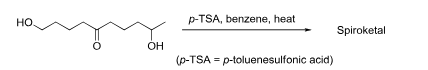
\includegraphics[width=0.55\columnwidth]{figs/q35.png}
    \caption{Figure for Q.35}
    \label{fig:q35}
\end{figure}

The most predominant spiroketal is  

\begin{figure}[H]
\centering
\begin{enumerate}
    \item 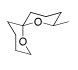
\includegraphics[width=0.18\columnwidth]{figs/q35a.png}
    \caption{Option A}
    \label{fig:q35a}
    \item 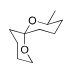
\includegraphics[width=0.18\columnwidth]{figs/q35b.png}
    \caption{Option B}
    \label{fig:q35b}
    \item 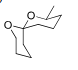
\includegraphics[width=0.18\columnwidth]{figs/q35c.png}
    \caption{Option C}
    \label{fig:q35c}
    \item 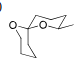
\includegraphics[width=0.18\columnwidth]{figs/q35d.png}
    \caption{Option D}
    \label{fig:q35d}
\end{enumerate}
\end{figure}
\hfill (GATE CY 2012)


\item For a face centered cubic lattice, the Miller indices for the first Bragg’s peak (smallest Bragg angle) are  

\begin{multicols}{2}
\begin{enumerate}
    \item 002
    \item 111
    \item 001
    \item 110
\end{enumerate}
\end{multicols}
\hfill (GATE CY 2012)


\item For the titration of a 10 mL (aq) solution of CaCO$_3$, 2 mL of 0.001 M Na$_2$EDTA is required to reach the end point.  
The concentration of CaCO$_3$ (assume molecular weight of CaCO$_3$ = 100) is  

\begin{multicols}{2}
\begin{enumerate}
    \item $5 \times 10^{-4}$ g/mL
    \item $2 \times 10^{-4}$ g/mL
    \item $5 \times 10^{-3}$ g/mL
    \item $2 \times 10^{-3}$ g/mL
\end{enumerate}
\end{multicols}
\hfill (GATE CY 2012)

\item In the reaction  

\begin{figure}[H]
    \centering
    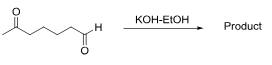
\includegraphics[width=0.55\columnwidth]{figs/q38.png}
    \caption{Figure for Q.38}
    \label{fig:q38}
\end{figure}

the product formed is  

\begin{figure}[H]
\centering
\begin{enumerate}
    \item 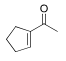
\includegraphics[width=0.20\columnwidth]{figs/q38a.png}
    \caption{Option A}
    \label{fig:q38a}
    \item 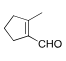
\includegraphics[width=0.20\columnwidth]{figs/q38b.png}
    \caption{Option B}
    \label{fig:q38b}
    \item 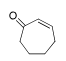
\includegraphics[width=0.20\columnwidth]{figs/q38c.png}
    \caption{Option C}
    \label{fig:q38c}
    \item 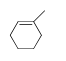
\includegraphics[width=0.20\columnwidth]{figs/q38d.png}
    \caption{Option D}
    \label{fig:q38d}
\end{enumerate}
\end{figure}
\hfill (GATE CY 2012)


\item In the reaction given below, identify the product  

\begin{figure}[H]
    \centering
    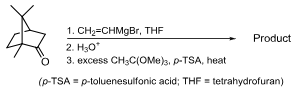
\includegraphics[width=0.60\columnwidth]{figs/q39.png}
    \caption{Figure for Q.39}
    \label{fig:q39}
\end{figure}

\begin{figure}[H]
\centering
\begin{enumerate}
    \item 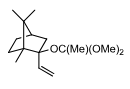
\includegraphics[width=0.22\columnwidth]{figs/q39a.png}
    \caption{Option A}
    \label{fig:q39a}
    \item 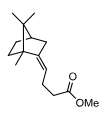
\includegraphics[width=0.22\columnwidth]{figs/q39b.png}
    \caption{Option B}
    \label{fig:q39b}
    \item 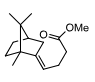
\includegraphics[width=0.22\columnwidth]{figs/q39c.png}
    \caption{Option C}
    \label{fig:q39c}
    \item 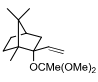
\includegraphics[width=0.22\columnwidth]{figs/q39d.png}
    \caption{Option D}
    \label{fig:q39d}
\end{enumerate}
\end{figure}
\hfill (GATE CY 2012)


\item Consider the following pairs of complexes  

\[
\begin{aligned}
&[\text{Co(NH}_3)_5\text{Br}]^{2+} \text{ and } [\text{Cr(OH}_2)_6]^{2+} 
&[\text{Co(NH}_3)_5(\text{OH})]^{2+} \text{ and } [\text{Cr(OH}_2)_6]^{2+} 
&[\text{Co(NH}_3)_6]^{3+} \text{ and } [\text{Cr(OH}_2)_6]^{2+} 
&[\text{Co(NH}_3)_6]^{2+} \text{ and } [\text{Cr(OH}_2)_6]^{2+}
\end{aligned}
\]

The electron transfer rate will be fastest in the pair  

\begin{enumerate}
\begin{multicols}{2}
\item \ce{[Co(NH3)5Br]^{2+} and [Cr(OH2)6]^{2+}}
\item \ce{[Co(NH3)5(OH)]^{2+} and [Cr(OH2)6]^{2+}}
\item \ce{[Co(NH3)6]^{3+} and [Cr(OH2)6]^{2+}}
\item \ce{[Co(NH3)6]^{2+} and [Cr(OH2)6]^{2+}}
\end{multicols}
\end{enumerate}
\hfill (GATE CY 2012)


\item The extent of M\"ossbauer quadrupole splitting of iron follows the order
\begin{enumerate}
\item FeCl$_2 \cdot 4$H$_2$O $>$ K$_2$[Fe(CN)$_5$(NO)] $>$ FeCl$_3 \cdot 6$H$_2$O
\item K$_2$[Fe(CN)$_5$(NO)] $>$ FeCl$_2 \cdot 4$H$_2$O $>$ FeCl$_3 \cdot 6$H$_2$O
\item FeCl$_3 \cdot 6$H$_2$O $>$ K$_2$[Fe(CN)$_5$(NO)] $>$ FeCl$_2 \cdot 4$H$_2$O
\item FeCl$_3 \cdot 6$H$_2$O $>$ FeCl$_2 \cdot 4$H$_2$O $>$ K$_2$[Fe(CN)$_5$(NO)]
\end{enumerate}
\hfill (GATE CY 2012)


\item Hemoglobin is an oxygen carrying protein. The correct statement about oxy-hemoglobin is that
\begin{enumerate}
\item the metal is low-spin in +3 oxidation state while dioxygen is in O$_2^-$ form
\item the metal is high-spin in +3 oxidation state while dioxygen is in O$_2^-$ form
\item the metal is low-spin in +3 oxidation state while dioxygen is in neutral form
\item the metal is high-spin in +3 oxidation state while dioxygen is in neutral form
\end{enumerate}
\hfill (GATE CY 2012)


\item If a mixture of NaCl, conc. H$_2$SO$_4$ and K$_2$Cr$_2$O$_7$ is heated in a dry test tube, a red vapour (P) is formed. This vapour (P) dissolves in aqueous NaOH to form a yellow solution, which upon treatment with AgNO$_3$, forms a red solid (Q). P and Q are, respectively
\begin{multicols}{2}
\begin{enumerate}
\item CrO$_2$Cl$_2$ and Ag$_2$CrO$_4$
\item Na[CrOCl$_5$] and Ag$_2$CrO$_7$
\item Na$_2$[CrOCl$_5$] and Ag$_2$Cr$_2$O$_7$
\item CrO$_2$Cl$_2$ and Ag$_2$CrO$_7$
\end{enumerate}
\end{multicols}
\hfill (GATE CY 2012)

\item For the following reaction
\[
2\text{MnO}_4^- + 5\text{H}_2\text{C}_2\text{O}_4 + 6\text{H}^+ \longrightarrow 2\text{Mn}^{2+} + 8\text{H}_2\text{O} + 10\text{CO}_2
\]
E$^\circ$(MnO$_4^-$/Mn$^{2+}$) = +1.51 V and E$^\circ$(CO$_2$/H$_2$C$_2$O$_4$) = –0.49 V. 
At 298 K, the equilibrium constant is
\begin{multicols}{2}
\begin{enumerate}
\item 10$^{100}$
\item 10$^{148}$
\item 10$^{48}$
\item 10$^{143}$
\end{enumerate}
\end{multicols}
\hfill (GATE CY 2012)
\degree

\item The ground states of high-spin octahedral and tetrahedral Co(II) complexes are, respectively
\begin{multicols}{2}
\begin{enumerate}
\item $^4T_{2g}$ and $^4A_2$
\item $^4T_{1g}$ and $^4A_2$
\item $^4T_{1g}$ and $^4T_2$
\item $^4T_{1g}$ and $^4T_1$
\end{enumerate}
\end{multicols}
\hfill (GATE CY 2012)


\item The INCORRECT statement about Zeise’s salt is
\begin{multicols}{2}
\begin{enumerate}
\item Zeise’s salt is diamagnetic
\item The oxidation state of Pt in Zeise’s salt is +2
\item All the Pt–Cl bond lengths in Zeise’s salt are equal
\item C–C bond length of ethylene moiety in Zeise’s salt is longer than that of free ethylene molecule
\end{enumerate}
\end{multicols}
\hfill (GATE CY 2012)


\item The number of possible isomers for the square planar mononuclear complex [(NH$_3$)$_2$M(CN)$_2$] of a metal M is
\begin{multicols}{2}
\begin{enumerate}
\item 2
\item 4
\item 6
\item 3
\end{enumerate}
\end{multicols}
\hfill (GATE CY 2012)

\section*{Common Data Questions}

Common Data for Questions 48 and 49: 
Consider the reaction sequence shown below:

\begin{figure}[H]
\centering
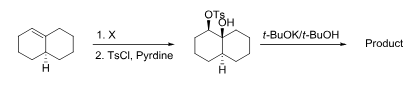
\includegraphics[width=0.6\columnwidth]{figs/q48-49.png} 
\caption{Figure for Q.48–49}
\label{fig:q48-49}
\end{figure}

TsCl = $p$-toluenesulfonyl chloride

\item The oxidant X used in step 1 is
\begin{multicols}{2}
\begin{enumerate}
\item CrO$_3$
\item OsO$_4$
\item NaIO$_4$
\item $m$-CPBA followed by NaOH
\end{enumerate}
\end{multicols}
\hfill (GATE CY 2012)

\item The product is
\begin{enumerate}
\item 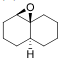
\includegraphics[width=0.25\columnwidth]{figs/q49a.png}
\captionsetup{hypcap=false}
\captionof{figure}{Option A}
\label{fig:q49a}

\item 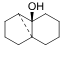
\includegraphics[width=0.25\columnwidth]{figs/q49b.png}
\captionof{figure}{Option B}
\label{fig:q49b}

\item 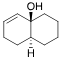
\includegraphics[width=0.25\columnwidth]{figs/q49c.png}
\captionof{figure}{Option C}
\label{fig:q49c}

\item 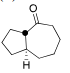
\includegraphics[width=0.25\columnwidth]{figs/q49d.png}
\captionof{figure}{Option D}
\label{fig:q49d}
\end{enumerate}
\hfill (GATE CY 2012)

{Common Data for Questions 50 and 51:} 
Consider the E1 reaction of \textit{tert}-amyl halides from the energy profile given below.

\begin{figure}[H]
    \centering
    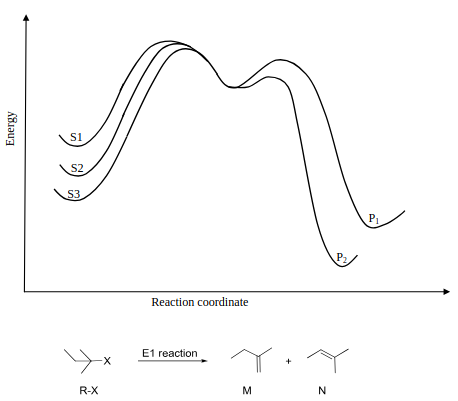
\includegraphics[width=0.65\columnwidth]{figs/q50.png}
    \caption{Figure for Q.50-51}
    \label{fig:q50}
\end{figure}


\item In the above reaction, X = Cl, Br or I. Based on the graph, identify the alkyl halides (R–X) as S$_1$, S$_2$ and S$_3$.

\begin{enumerate}
    \item S$_1$ = R–Cl,  S$_2$ = R–Br and S$_3$ = R–I
    \item S$_1$ = R–I,  S$_2$ = R–Br and S$_3$ = R–Cl
    \item S$_1$ = R–Cl,  S$_2$ = R–I and S$_3$ = R–Br
    \item S$_1$ = R–I,  S$_2$ = R–Cl and S$_3$ = R–Br
\end{enumerate}
\hfill (GATE CY 2012)

\item Identify product P$_1$, and its yield relative to P$_2$.

\begin{enumerate}
    \item P$_1$ is M and is the major product
    \item P$_1$ is N and is the minor product
    \item P$_1$ is N and is the major product
    \item P$_1$ is M and is the minor product
\end{enumerate}
\hfill (GATE CY 2012)

\textbf{Linked Answer Questions}

\textbf{Statement for Linked Answer Questions 52 and 53:}
A 20491 cm$^{-1}$ laser line was used to excite oxygen molecules (made of $^{16}$O only) to obtain the rotational Raman spectrum. The resulting rotational Raman spectrum of oxygen molecule has the first Stokes line at 20479 cm$^{-1}$.

    \item The rotational constant (usually denoted as $B$) for the oxygen molecule is

    \begin{multicols}{2}
    \begin{enumerate}
        \item 1.2 cm$^{-1}$
        \item 2.0 cm$^{-1}$
        \item 3.0 cm$^{-1}$
        \item 6.0 cm$^{-1}$
    \end{enumerate}
    \end{multicols}
    \hfill (GATE CY 2012)

    \item The next rotational Stokes line is expected at

    \begin{multicols}{2}
    \begin{enumerate}
        \item 20467 cm$^{-1}$
        \item 20469 cm$^{-1}$
        \item 20471 cm$^{-1}$
        \item 20475 cm$^{-1}$
    \end{enumerate}
    \end{multicols}
    \hfill (GATE CY 2012)


\textbf{Statement for Linked Answer Questions 54 and 55:}
Hückel molecular orbital theory can be applied to the allene radical
\[
\text{CH}_2=\text{CH}-\text{CH}_2
\]

\item The secular determinant (where $\alpha$, $\beta$ and $E$ have their usual meanings) is given by

    \begin{multicols}{2}
    \begin{enumerate}
        \item $\myvec{
    \alpha - E & \beta & 0 \\
    \beta & \alpha - E & \beta \\
    0 & \beta & \alpha - E
}$

\item $\myvec{
    \alpha - E & 0 & 0 \\
    0 & \alpha - E & \beta \\
    0 & \beta & \alpha - E
}$

\item $\myvec{
    \alpha - E & \beta & 0 \\
    \beta & \alpha - E & 0 \\
    0 & \beta & \alpha - E
}$

\item $\myvec{
    \alpha - E & -\beta & 0 \\
    -\beta & \alpha - E & -\beta \\
    0 & -\beta & \alpha - E
}$

    \end{enumerate}
    \end{multicols}
    \hfill (GATE CY 2012)

\item The possible values of $E$ are
\begin{enumerate}
    \item $\alpha + \sqrt{2}\beta, \, \alpha, \, \alpha - \sqrt{2}\beta$
    \item $\alpha + 2\sqrt{2}\beta, \, \alpha, \, \alpha - 2\sqrt{2}\beta$
    \item $\alpha + \beta, \, \alpha, \, \alpha - \beta$
    \item $\alpha + 2\beta, \, \alpha, \, \alpha - 2\beta$
\end{enumerate}
\hfill (GATE CY 2012)

\section*{General Aptitude (GA) Questions (Compulsory)}

\textbf{Q. 56 -- Q. 60 carry one mark each.}


\item If $(1.001)^{129} = 3.52$ and $(1.001)^{284} = 7.85$, then $(1.001)^{4241} =$ 

\begin{multicols}{2}
\begin{enumerate}
    \item 2.23
    \item 4.33
    \item 11.37
    \item 27.64
\end{enumerate}
\end{multicols}
\hfill (GATE CY 2012)

\item One of the parts (A, B, C, D) in the sentence given below contains an ERROR. Which one of the following is \textbf{INCORRECT}?

\textbf{I requested that he should be given the driving test today instead of tomorrow.}

\begin{multicols}{2}
\begin{enumerate}
    \item requested that
    \item should be given
    \item the driving test
    \item instead of tomorrow
\end{enumerate}
\end{multicols}
\hfill (GATE CY 2012)

\item Which one of the following options is the closest in meaning to the word given below?

\textbf{Latitude}

\begin{multicols}{2}
\begin{enumerate}
    \item Eligibility
    \item Freedom
    \item Coercion
    \item Meticulousness
\end{enumerate}
\end{multicols}
\hfill (GATE CY 2012)

\item Choose the most appropriate word from the options given below to complete the following sentence:

\textbf{Given the seriousness of the situation that he had to face, his \_\_\_ was impressive.}

\begin{multicols}{2}
\begin{enumerate}
    \item beggary
    \item nomenclature
    \item jealousy
    \item nonchalance
\end{enumerate}
\end{multicols}
\hfill (GATE CY 2012)

\item Choose the most appropriate alternative from the options given below to complete the following sentence:

\textbf{If the tired soldier wanted to lie down, he \_\_\_ the mattress out on the balcony.}

\begin{multicols}{2}
\begin{enumerate}
    \item should take
    \item shall take
    \item should have taken
    \item will have taken
\end{enumerate}
\end{multicols}
\hfill (GATE CY 2012)

\textbf{Q. 61 -- Q. 65 carry two marks each.}


\item \textbf{One of the legacies of the Roman legions was discipline. In the legions, military law prevailed and discipline was brutal. Discipline on the battlefield kept units obedient, intact and fighting, even when the odds and conditions were against them.}

Which one of the following statements best sums up the meaning of the above passage?

\begin{enumerate}
    \item Thorough regimentation was the main reason for the efficiency of the Roman legions even in adverse circumstances.
    \item The legions were treated inhumanly as if the men were animals.
    \item Discipline was the armies’ inheritance from their seniors.
    \item The harsh discipline to which the legions were subjected led to the odds and conditions being against them.
\end{enumerate}
\hfill (GATE CY 2012)

    \item A and B are friends. They decide to meet between 1 PM and 2 PM on a given day. There is a condition that whoever arrives first will not wait for the other for more than 15 minutes. The probability that they will meet on that day is
    \begin{multicols}{2}
        \begin{enumerate}
            \item $\dfrac{1}{4}$
            \item $\dfrac{1}{16}$
            \item $\dfrac{7}{16}$
            \item $\dfrac{9}{16}$
        \end{enumerate}
    \end{multicols}
    \hfill (GATE CY 2012)

    \item The data given in the following table summarizes the monthly budget of an average household.

    \begin{tabular}[12pt]{ |c| c| c| c| }
\hline
$\beta$ & Airplane A & Airplane B & Airplane C \\
\hline
$\beta = -5\,\mathrm{deg}$ & $-0.030$ & $-0.025$ & $0.040$\\
\hline
$\beta = 0\,\mathrm{deg}$ & $0$ & $0$ & $0$ \\
\hline
$\beta = 5\,\mathrm{deg}$ & $0.030$ & $0.025$ & $-0.040$\\
\hline
\end{tabular}

    \captionsetup{type=table}
\captionof{table}{Table for Q.63}

    

    The approximate percentage of the monthly budget NOT spent on savings is
    \begin{multicols}{2}
        \begin{enumerate}
            \item 10\%
            \item 14\%
            \item 81\%
            \item 86\%
        \end{enumerate}
    \end{multicols}
    \hfill (GATE CY 2012)

    \item There are eight bags of rice looking alike, seven of which have equal weight and one is slightly heavier. The weighing balance is of unlimited capacity. Using this balance, the minimum number of weighings required to identify the heavier bag is
    \begin{multicols}{2}
        \begin{enumerate}
            \item 2
            \item 3
            \item 4
            \item 8
        \end{enumerate}
    \end{multicols}
    \hfill (GATE CY 2012)

    \item Raju has 14 currency notes in his pocket consisting of only Rs. 20 notes and Rs. 10 notes. The total money value of the notes is Rs. 230. The number of Rs. 10 notes that Raju has is
    \begin{multicols}{2}
        \begin{enumerate}
            \item 5
            \item 6
            \item 9
            \item 10
        \end{enumerate}
    \end{multicols}
    \hfill (GATE CY 2012)


\begin{center}
\textbf{END OF THE QUESTION PAPER}
\end{center}



\end{enumerate}
\end{document}
     
